\documentclass{article}

\usepackage[utf8]{inputenc}   %	Zeichencodierung nach UTF-8 (Unicode)
\usepackage[T1]{fontenc}
\usepackage{lmodern}
\usepackage[T1]{url}
\usepackage[final]{graphicx}
\usepackage[automark]{scrlayer-scrpage}
\usepackage{setspace}

\usepackage[plainpages=false,pdfpagelabels,hypertexnames=false]{hyperref}

\usepackage{amsmath}
\usepackage{caption}
\usepackage{subcaption}

% cref
\usepackage{cleveref}
\creflabelformat{equation}{#2\textup{#1}#3}

% tikz graphs and state machines
\usepackage{tikz}
\usetikzlibrary{automata,arrows,calc,positioning}

%circuitikz
\usepackage[siunitx]{circuitikz}

\title{Un0rick Anti Aliasing Low Pass Filter}
\author{Tim Treichel}

\begin{document}
\maketitle
The electrical signal that is generated by the piezoelectric receiver is run through a single ended wire to the \textbf{AD8331} VGA. The output of the amplifier is a differential signal, which is filtered by a differential anti-aliasing low pass filter(\cref{fig:un0rick_circuit_filter_diff}). Beside the schematics of the board, no official documentation of this filter is released. However, in the field of measurement and signal processing, this could be important information.
Therefore the anti-aliasing filter was calculated and independently simulated with spice. 

First the differential filter (\cref{fig:un0rick_circuit_filter_diff}) was transformed into a single ended filter (\cref{fig:un0rick_circuit_filter_single}). This transformation can be applied by removing the horizontal components of one end (in this case $R_{1'}$,$L_{1'}$, $C_{1'}$ and $R_{2'}$ were removed), while keeping the horizontal components of the other end unchanged. The capacity of the vertical shunt capacitor in the differential circuit is half of the capacitor in the single ended circuit, therefore the capacity of $C_2$ has to doubled during the transformation.

The corresponding single ended filter has the same properties, i.e. the same transfer function, as the differential filter. The transfer function $H(s)$ was calculated on the basis of the simplified single ended circuit (\cref{fig:un0rick_circuit_filter_single}) following the \cref{eq:Hs1,eq:Hs2,eq:Hs3,eq:Hs4,eq:Hs5,eq:Hs6,eq:Hs7}. 

To verify the accuracy of the calculated transfer function (\cref{eq:Hs7}) as well as the transformation from the differential filter to a single ended filter, both circuits (\cref{fig:un0rick_circuit_filter_diff,,fig:un0rick_circuit_filter_single}) were simulated in spice (\emph{ngspice}) and the corresponding bode plots are visualized in \cref{fig:un0rick_aa_filter_bode_spice}. It is notable, that in order to distinguish between the different plots a small offset (y-axis) is added for each new line. The plots are all similar enough to assume that the transformation and calculations are correct.\\

\noindent When looking at the frequency response of the bode plot (\cref{fig:un0rick_aa_filter_bode_spice}) the low pass characteristic is of this filter is obvious. The gain is constant throughout the lower frequencies until it peaks around $40 \, MHz$ after which it drops. The cutoff frequency at $-3 \, dB$ is at around $65 \, MHz$ (see \cref{fig:un0rick_aa_filter_cutoff}). This is unexpectedly high, since the sampling rate of the ADC is $64 \, MHz$, which usually is combined, with a cutoff frequency half as big. 

The cutoff frequency is higher then the \emph{Nyquist frequency} of the ADC, therefore, in theory, aliasing can occur. In reality it probably is not very likely for the aliasing to occur in the form of ultrasonic waves, as long as common transducers are used, because the frequency range between $32 \, MHz$ and $64 \, MHz$ (in which the aliasing can occur), is not part of the signal bandwidth and therefore should mostly contain low level noise. However measurements with ultra-high-frequency ultrasonic transducers could experience aliasing with the currently implemented filter. Furthermore aliasing can always occur on the electrical signal trays, especially since the un0rick board has high frequency analog signals as well as high frequency digital signals (FPGA) on the same board.

It is also notable that this filter is not a standard filter like i.e. a Butterworth or Chebyshev filter. It is more likely based on the low pass filter circuits shown in the data sheet of the \textbf{AD8331}.

Based on the calculated transfer function (\cref{eq:Hs7}), the characteristics of the filter were calculated. As mentioned above, the bode plot (\cref{fig:un0rick_aa_filter_bode_spice}) shows the magnitude (\cref{eq:aa_filter_amplitude} in dB) and phase (\cref{eq:aa_filter_phase}) of the frequency response (\cref{eq:aa_filter_fresponse}), while \cref{fig:un0rick_aa_filter_cutoff} shows the magnitude around the cutoff frequency. Group and phase delay (\cref{eq:aa_filter_group_delay,,eq:aa_filter_phase_delay}) are plotted in \cref{fig:un0rick_aa_filter_group_delay,,fig:un0rick_aa_filter_phase_delay} respectively. The plots for the magnitude, phase and impulse response (\cref{fig:un0rick_aa_filter_impulse}) were calculated by the use of the python \emph{SciPy} signal processing library.

\begin{figure}
	\centering
	\begin{circuitikz}
		\draw
		(0,5) to [short, *-*]  (2,5)
		(2,5) -- (2,6) to [R, l=$R_1$\text{ = 100 $\Omega$}] (4,6) -- (4,5)
		(2,5) -- (2,4) to [L, l_=$L_1$\text{ = 100 nH}] (4,4) -- (4,5)
		(4,5) to [C,l=$C_1$\text{ = 100 nF}, *-] (7,5) to [R,l=$R_2$\text{ = 18 $\Omega$}, -*] (9,5) to [short, -*] (12,5)
		(9,5) to [C,l=$C_2$\text{ = 50 pF}] (9,1) to [short, *-*] (12,1)
		(0,1) to [short, *-*]  (2,1)
		(2,1) -- (2,2) to [R, l=$R_{1'}$\text{ = $R_1$}] (4,2) -- (4,1)
		(2,1) -- (2,0) to [L, l_=$L_{1'}$\text{ = $L_1$}] (4,0) -- (4,1)
		(4,1) to [C,l=$C_{1'}$\text{ = $C_1$}, *-] (7,1) to [R,l=$R_{2'}$\text{ = $R_2$}, -*] (9,1) to [short, -*] (12,1)
		(-0.5,5) node[]{\text{$U_{in+}$}}
		(-0.5,1) node[]{\text{$U_{in-}$}}
		(12.7,5)   node[]{\text{$U_{out+}$}}
		(12.7,1)   node[]{\text{$U_{out-}$}}
		;
	\end{circuitikz}
	\caption{Differential anti-aliasing low pass filter}
		\label{fig:un0rick_circuit_filter_diff}
\end{figure}

\begin{figure}
	\centering
	\begin{circuitikz}
		\draw
		(0,4) to [short, *-*]  (2,4)
		(2,4) -- (2,5) to [R, l=$R_1$\text{ = 100 $\Omega$}] (4,5) -- (4,4)
		(2,4) -- (2,3) to [L, l_=$L_1$\text{ = 100 nH}] (4,3) -- (4,4)
		(4,4) to [C,l=$C_1$\text{ = 100 nF}, *-] (7,4) to [R,l=$R_2${ = 18 $\Omega$}, -*] (9,4) to [short, -*] (12,4)
		(9,4) to [C,l=$C_2$\text{ = 100 pF}] (9,0) to [short, *-*] (12,0)
		(0,0) to [short, *-] (9,0)
		(0,0) to [open, v^>=$U_{input}$]  (0,4) 
		(12,4) to [open, v^>=$U_{output}$] (12,0) 
		;
	\end{circuitikz}
	\caption{Single ended anti-aliasing low pass filter after transformation}
	\label{fig:un0rick_circuit_filter_single}
\end{figure}


\begin{align}
	%-------------------------------------
	%
	H(s) &= \frac{U_{output}}{U_{input}}\label{eq:Hs1}\\
	%
	%-------------------------------------
	%
	H(s) &= \frac{Z_3}{Z_1 + Z_2 + Z_3} \;\; \text{with } Z_1 = \frac{sL_1R_1}{sL_1 + R_1} \;,\; Z_2 = R_2 + \frac{1}{sC_1} \;,\; Z_3 = \frac{1}{sC_2}\label{eq:Hs2}\\
	%
	%-------------------------------------
	%
	H(s) &= \frac{\frac{1}{sC_2}}{[\frac{sL_1R_1}{sL_1 + R_1}] + [R_2 + \frac{1}{sC_1}] + [\frac{1}{sC_2}]}\label{eq:Hs3}\\
	%
	%-------------------------------------
	%
	H(s) &= \frac{1}{[\frac{s^2C_2L_1R_1}{sL_1 + R_1}] + [sC_2R_2] + [\frac{C_2}{C_1} + 1]}\label{eq:Hs4}\\
	%
	%-------------------------------------
	%
	H(s) &= \frac{sL_1 + R_1}{[s^2C_2L_1R_1] + [s^2C_2L_1R_2 + sC_2R_1R_2] + [s(\frac{C_2}{C_1} + 1)L_1 + (\frac{C_2}{C_1} + 1)R_1]}\label{eq:Hs5}\\
	%
	%-------------------------------------
	%
	H(s) &= \frac{sL_1 + R_1}{s^2C_2L_1(R_1+R_2) + s(C_2R_1R_2 + (\frac{C_2}{C_1} + 1)L_1) + (\frac{C_2}{C_1} + 1)R_1}\label{eq:Hs6}
	%
	%-------------------------------------
\end{align}

\noindent\begin{minipage}{.5\linewidth}
	\begin{align}
		\intertext{Transfer Funtion:}
		H(s) = \frac{sy_1 + y_0}{s^2x_2 + sx_1 + x_0} && \text{with }\nonumber\\\nonumber\\\nonumber
	\end{align}
\end{minipage}%
\begin{minipage}{.5\linewidth}
	\begin{align}
		\begin{split}
			y_1 &= L_1 \\
			y_0 &= R_1 \\
			x_2 &= C_2L_1(R_1+R_2) \\
			x_1 &= C_2R_1R_2 + (\frac{C_2}{C_1} + 1)L_1 \\
			x_0 &= (\frac{C_2}{C_1} + 1)R_1
		\end{split}\label{eq:Hs7}
	\end{align}
\end{minipage}

\begin{align}
	%-------------------------------------
	%
	\intertext{Frequency Response:}
	H(j\omega) &= \frac{j\omega y_1 + y_0}{-\omega^2x_2 + j\omega x_1 + x_0}\\
	H(j\omega) &= \frac{y_0 + j\omega y_1}{(x_0 - \omega^2x_2) + j\omega x_1}\label{eq:aa_filter_fresponse}
	%
	%-------------------------------------
	%
	\intertext{Amplitude:}
	|H(j\omega)| &= \frac{\sqrt{y_0^2 + (\omega y_1)^2}}{\sqrt{(x_0 - \omega^2x_2)^2 + (\omega x_1)^2}}\label{eq:aa_filter_amplitude}
	%
	%-------------------------------------
	%
	\intertext{Phase:}
	\phi(\omega) &= arg\{H(j\omega)\}\\
	\phi(\omega) &= arctan(\frac{\omega y_1}{y_0}) - arctan(\frac{\omega x_1}{x_0 - \omega^2x_2})\label{eq:aa_filter_phase}
	%
	%-------------------------------------
	%
	\intertext{Group Delay:}
	\tau_{g}(\omega) &= - \frac{d\phi(\omega)}{d\omega}\\
	\tau_{g}(\omega) &= \frac{x_1 (\omega^2 x_2 + x_0)}{\omega^4 x_2^2  + \omega^2 x_1^2 - 2 \omega^2 x_0 x_2 + x_0^2} - \frac{y_0 y_1}{\omega^2 y_1^2 + y_0^2}\label{eq:aa_filter_group_delay}
	%
	%-------------------------------------
	%
	\intertext{Phase Delay:}
	\tau_{\phi}(\omega) &= - \frac{\phi(\omega)}{\omega}\\
	\tau_{\phi}(\omega) &= \frac{arctan(\frac{\omega x_1}{x_0 - \omega^2x_2}) - arctan(\frac{\omega y_1}{y_0})}{\omega}\label{eq:aa_filter_phase_delay}
	%
	%-------------------------------------
\end{align}

\begin{figure}
	\centering
	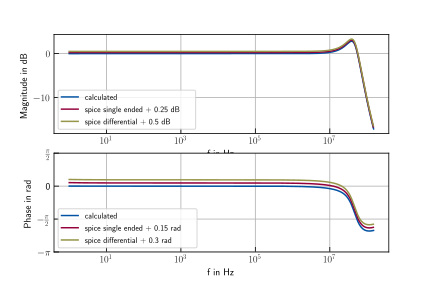
\includegraphics[width=\linewidth]{Images/pdf/un0rick_aa_filter_bode}
	\caption{Bode plot of calculated transfer function and simulated (spice) circuits}
	\label{fig:un0rick_aa_filter_bode_spice}
\end{figure}

\begin{figure*}
	\centering
	\begin{subfigure}[b]{0.475\textwidth}
		\centering
		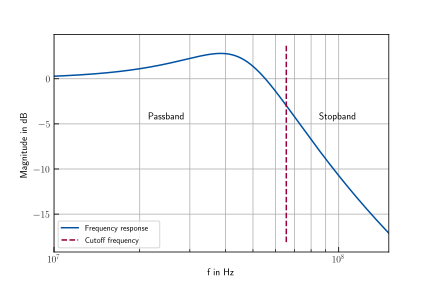
\includegraphics[width=\textwidth]{Images/pdf/un0rick_aa_filter_fresponse_mag_cutoff}
		\caption{\centering Frequency response with cutoff frequency}
		\label{fig:un0rick_aa_filter_cutoff}
	\end{subfigure}
	\hfill
	\begin{subfigure}[b]{0.475\textwidth}
		\centering
		\includegraphics[width=\textwidth]{Images/pdf/un0rick_aa_filter_impulse}
		\caption{\centering Impulse response \newline}
		\label{fig:un0rick_aa_filter_impulse}
	\end{subfigure}	
	\vskip\baselineskip
	\begin{subfigure}[b]{0.475\textwidth}
		\centering
		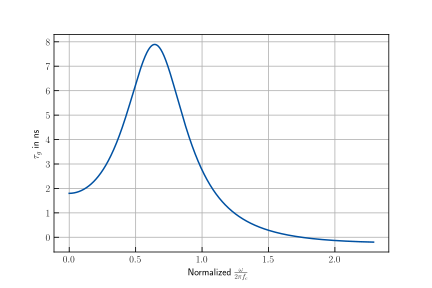
\includegraphics[width=\textwidth]{Images/pdf/un0rick_aa_filter_group_delay}
		\caption{\centering Group delay}
		\label{fig:un0rick_aa_filter_group_delay}
	\end{subfigure}
	\hfill
		\begin{subfigure}[b]{0.475\textwidth}
		\centering
		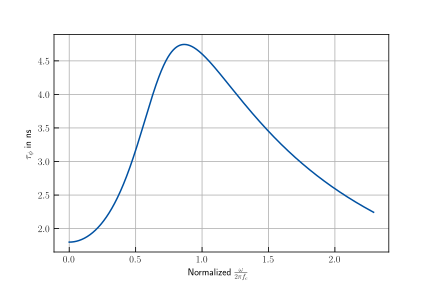
\includegraphics[width=\textwidth]{Images/pdf/un0rick_aa_filter_phase_delay}
		\caption{\centering Phase delay}
		\label{fig:un0rick_aa_filter_phase_delay}
	\end{subfigure}

	\caption{\centering More characteristics of the un0rick anti-aliasing low pass filter} 
	\label{fig:un0rick_aa_characteristics}
\end{figure*}
\end{document}